\section{\textbf{Dependencies in Dyadic Data}}

When modeling dyadic data scholars typically employ a generalized linear model (GLM) estimated via maximum-likelihood. This type of model is expressed via a stochastic and systematic component \citep{pawitan:2013}. The stochastic component reflects our assumptions about the probability distribution from which the data are generated: $y_{ij} \sim P(Y | \theta_{ij})$, with a probability density or mass function, such as the normal, binomial, or Poisson, and we assume that each dyad in the sample is independently drawn from that particular distribution, given $\theta_{ij}$. The systematic component characterizes the model for the parameters of that distribution and describes how $\theta_{ij}$ varies as a function of a set of nodal and dyadic covariatse, $\mathbf{X_{ij}}$: $\theta_{ij} = \bm\beta^{T} \mathbf{X}_{ij}$. A fundamental assumption we make when applying this modeling technique is that given $\mathbf{X}_{ij}$ and the parameters of our distribution, each of the dyadic observations are conditionally independent. The importance of this assumption becomes clearer in the process of estimating a GLM via maximum likelihood. After having chosen a set of covariates and specifying a distribution, we construct the joint density function over all dyads, for example:

\vspace{-8mm}
\begin{align}
\begin{aligned}
	P(y_{ij}, y_{ik}, \ldots | \theta_{ij}, \theta_{ik}, \ldots ) &= P(y_{ij} | \theta_{ij}) \times P(y_{ik} | \theta_{ik}) \times \ldots  \\
	P(\mathbf{Y} \; | \; \bm{\theta}) &= \prod_{\alpha=1}^{n \times (n-1)} P(y_{\alpha} | \theta_{\alpha})  \\
\end{aligned}
\end{align}

\noindent We next convert the joint probability into a likelihood: $\displaystyle \mathcal{L} (\bm{\theta} | \mathbf{Y}) = \prod_{\alpha=1}^{n \times (n-1)} P(y_{\alpha} | \theta_{\alpha})$.

We can then estimate the parameters by maximizing the likelihood, or, more typically, the log-likelihood. However, the likelihood as defined above is only valid if we are able to make the assumption that, for example, $y_{ij}$ is independent of $y_{ji}$ and $y_{ik}$ given the set of covariates we specified, or the values of $\theta_{ij}$. Without the assumption of conditional observational independence the joint density function cannot be written in the way described above and a valid likelihood does not exist. Accordingly, inferences drawn from misspecified models that ignore potential interdependencies between dyadic observations are likely to have a number of issues including biased estimates of the effect of independent variables, uncalibrated confidence intervals, and poor predictive performance. The importance of accounting for the underlying structure of our data has been a lesson well understood, at least when it comes to time-series cross-sectional data (TSCS) within political science \citep{beck:katz:1995,beck:etal:1998}. As a result, it is now standard practice to take explicit steps to account for the complex data structures that emerge in TSCS applications and the unobserved heterogeneity that they cause.

% Scholars working with dyadic data typically begin by stacking observations associated with each dyad on top of one another and not passing any auxiliary information to the model about how observations may be interdependent. For example, in this design, a conflict initiated from the United States against Japan is assumed to be independent of any conflictual action that Japan may send to the United States. Additionally, every action sent by Japan to others in the system is considered independent even though each of those interactions involves a common sender, i.e, Japan. While most scholars begin with the assumption that each dyadic interaction takes place in isolation of the others, we know this assumption to be false both in theory and in practice. Relational data comes with an explicit structure that generally leads to particular types of dependencies. The importance of accounting for the underlying structure of our data has been a lesson well understood, at least when it comes to time-series cross-sectional data (TSCS) within political science \citep{beck:katz:1995,beck:etal:1998}. As a result, it is now standard practice to take explicit steps to account for the complex data structures that emerge in TSCS applications and the unobserved heterogeneity that they cause.

To uncover the underlying structure of relational data, it is helpful to restructure dyadic data in the form of a matrix---often referred to as an adjacency matrix---as shown in Figure~\ref{fig:adjMatDeps}. Rows designate the senders of an event and columns the receivers. The cross-sections in this matrix represent the actions that were sent by an actor in the row to those designated in the columns. Thus $y_{ij}$ designates an action $y$, such as a conflictual event or trade flow, that is sent from actor $i$ to actor $j$. In many applications, scholars are interested in studying undirected (i.e., symmetric) outcomes in which there is no clear sender or receiver, these type of outcomes still can, and we argue should, be studied using the type of framework we discuss below.

Using the structure of an adjacency matrix, Figure~\ref{fig:adjMatDeps} visualizes the types of first- and second-order dependencies that can complicate the analysis of relational data in traditional GLMs. The adjacency matrix on the top left highlights a particular row to illustrate that these values may be more similar to each other than other values because each has a common sender. Interactions involving a common sender also manifest heterogeneity in how active actors are across the network when compared to each other. In most relational datasets (e.g., trade flows, conflict, participation in international organizations, even networks derived from Twitter or Facebook), we often find that there are some actors that are much more active than others \citep{barabasi:reka:1999}. For example, in an analysis of international trade certain countries (e.g., China) export much larger volumes than other countries for a variety of structural, contextual, and idiosyncratic reasons. Unless one is able to develop a model that can account for the variety of explanations that may play a role in determining why a particular actor is more active than others, parameter estimates from standard statistical models will be biased.\footnote{In an undirected setting instead of studying sender and receiver heterogeneity, we would just be concerned with actor heterogeneity in general.}

\begin{figure}
	\begin{tabular}{cc}
		\textsc{Sender Heterogeneity} & \textsc{Receiver Heterogeneity} \\
		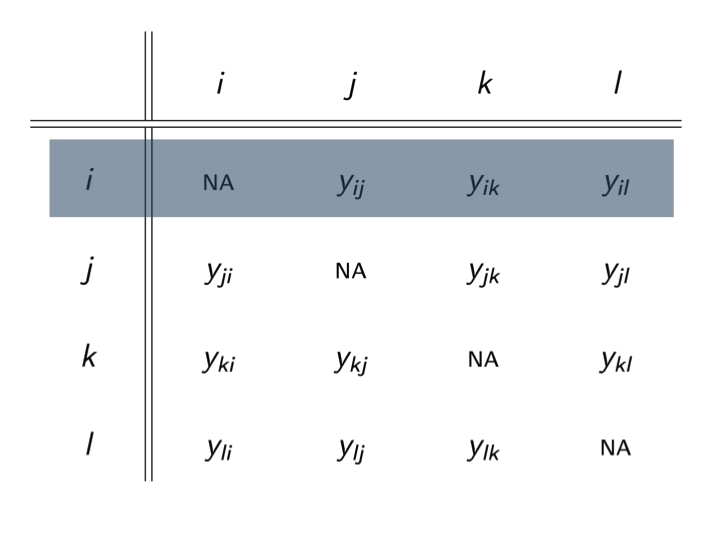
\includegraphics[width=.4\textwidth]{graphics/adjRowDep.png} &
		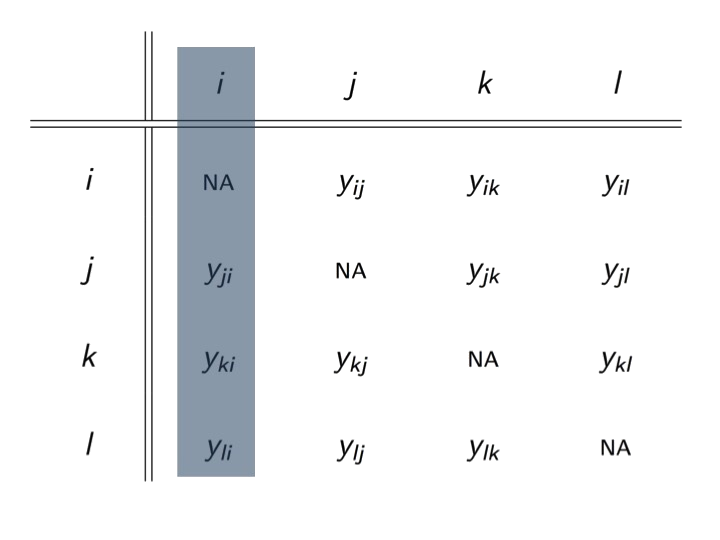
\includegraphics[width=.4\textwidth]{graphics/adjColDep.png} \\
		\textsc{Sender-Receiver Covariance} & \textsc{Reciprocity} \\
		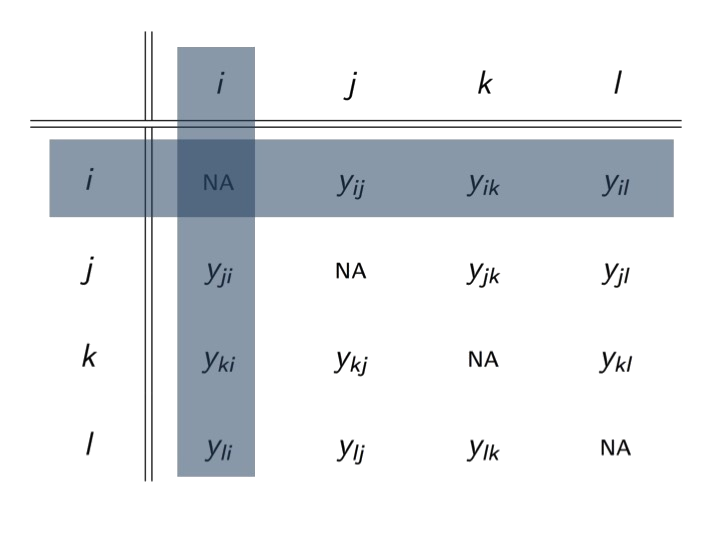
\includegraphics[width=.4\textwidth]{graphics/adjRowColCovar.png} &
		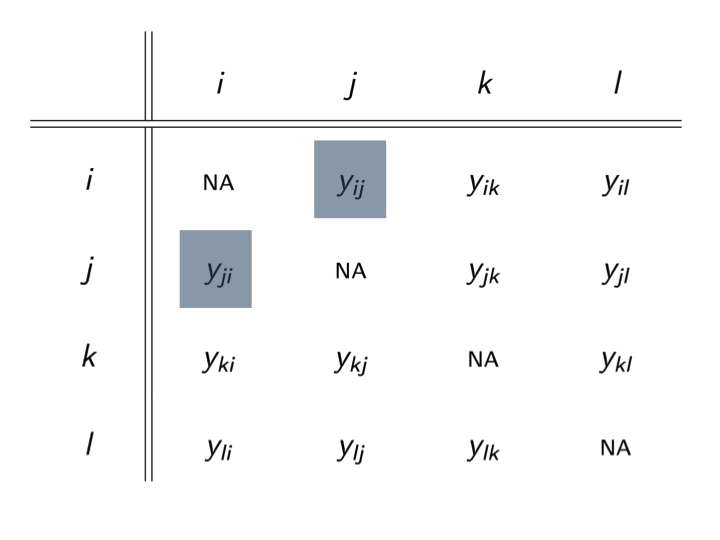
\includegraphics[width=.4\textwidth]{graphics/adjRecip.png} \\
	\end{tabular}
	\caption{Nodal and dyadic dependencies in relational data.}
	\label{fig:adjMatDeps}
\end{figure}

For similar reasons one also needs to take into account the dependence between observations that share a common receiver. The bottom-left panel in Figure~\ref{fig:adjMatDeps} illustrates that sender and receiver type dependencies can also blend together. Specifically, actors who are more likely to send ties in a network tend to also be more likely to receive them. As a result, the rows and columns in an adjacency matrix are often correlated. For example, consider trade flows both from and to many wealthy, developed countries. The bottom-right panel highlights a second-order dependence, specifically, reciprocity. This is a dependency occurring within dyads involving the same actors whereby values of $y_{ij}$ and $y_{ji}$ are correlated. The concept of reciprocity has deep roots in the study of relations between states \citep{richardson:1960,keohane:1989}.

For most relational data, however, dependencies do not simply manifest at the nodal or dyadic level. More often we find significant evidence of higher-order structures that result from dependencies between multiple groups of actors. These dependencies arise because there may be a set of latent attributes between actors that affects their probability of interacting with one another \citep{zinnes:1967,wasserman:faust:1994}. In Figure~\ref{fig:thirdDeps} we provide a visualization of a simulated relational dataset wherein the nodes designate actors and edges between the nodes indicate that an interaction between the two took place. To highlight third-order dependence patterns, nodes with similar latent attributes are colored similarly.

\begin{figure}[ht]
	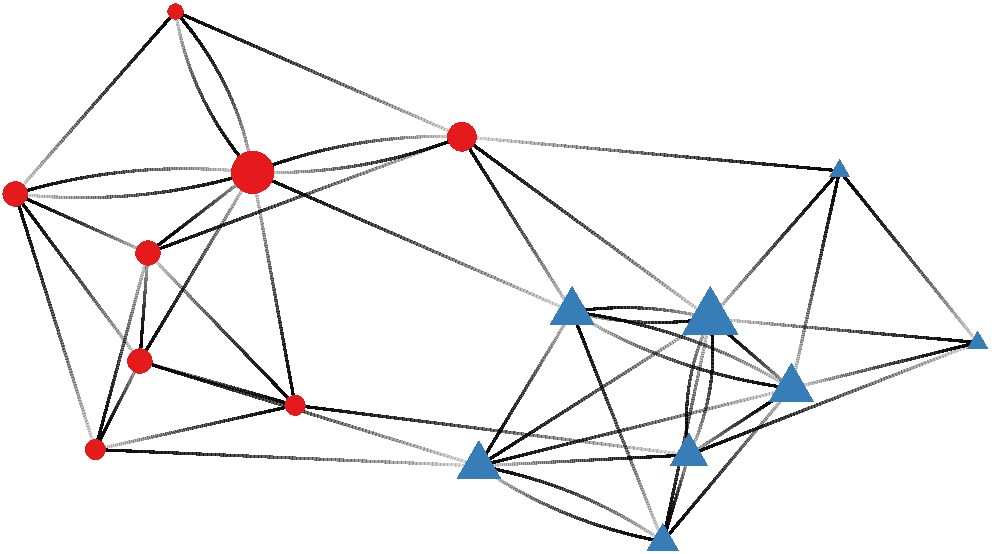
\includegraphics[width=.6\textwidth]{graphics/stochEquiv_v2.pdf}
	\caption{Higher-order dependence patterns in a network.}
	% need a simpler caption here
	\label{fig:thirdDeps}
\end{figure}

The visualization illustrates that actors belonging to the same group have a higher likelihood of interacting with each other, whereas interactions across groups are rarer. A prominent example of a network with this type of structure is discussed by \citet{adamic:glance:2005}, who visualize linkages between political blogs preceding the 2004 United States Presidential Election. \citeauthor{adamic:glance:2005} find that the degree of interaction between right- and left-leaning blogs is minimal and that most blogs are linked to others that are politically similar. This showcases the types of higher-order dependencies that can emerge in relational data. First, the fact that interactions are determined by a shared attribute, in this case political ideology, is an example of \textit{homophily}. Homophily explains the emergence of patterns such as transitivity (``a friend of a friend is a friend'') and balance (``an enemy of a friend is an enemy''), which also have a long history in international relations. The other major type of meso-scopic features that emerge in relational data is community structure \citep{mucha:etal:2010}, which is often formalized through the concept of stochastic equivalence \citep{anderson:etal:1992}. Stochastic equivalence refers to a type of pattern in which actors can be divided into groups such that members of the same group have similar patterns of relationships. In the example above, each of the left leaning blogs would be considered stochastically equivalent to one another because any given left-leaning blog is more likely to interact with a blog of a similar political position and less likely to interact with one of a divergent political position.

These types of patterns frequently emerge in IR contexts.\footnote{For example, see: \citet{manger:etal:2012, kinne:2013, chyzh:2016}.} For example, a perennial finding in the interstate trade literature emphasizes the role that geography plays in determining trade flows. Geographic proximity in the network context is an example of homophily---a shared attribute between actors that corresponds to a greater likelihood of the event of interest taking place. Alternatively, in the interstate conflict literature, we may find that actors who are each a member of a particular (formal or informal) alliance are likely to act similarly in the conflict network. Specifically, they will tend to initiate conflictual events with actors that their fellow alliance members initiate conflict with, and they will be unlikely to initiate conflict with members of their alliance---an example of stochastic equivalence. In both these examples, we are able to explicitly parameterize the attribute that might explain the emergence of higher order dependence patterns. While sometimes the conditions driving these patterns, such as geography, are easy to identify, at other times it can be difficult to describe exactly why higher order dependence patterns in networks may develop.

% International Trade, we might observe homophily wherein states with open economies and an absence of Non-Tariff Barriers are more likely to trade with each-other all else equal; alternatively we might observe heterophily in the sense that states that have greater endowments of capital are more likely to trade with states with greater endowments of land or labor.

%  We would also likely observe stochastic equivalence in an interstate war network wherein countries who are in conflict with the same target country are unlikely to fight one another. In this case, countries with (formal or informal) alliances are a member of the same group due to similar conflictual ties to other actors in the system.

\section{\textbf{Additive and Multiplicative Effect Models for Networks}}

To account for the dependencies that are prevalent in dyadic data, we turn to the AME model. The AME approach can be used to conduct inference on cross-sectional and longitudinal networks with binary, ordinal, or continuous linkages. It is flexible and easy to use for analyzing the kind of relational data often found in the social sciences. It accounts for nodal and dyadic dependence patterns, as well as higher-order dependencies such as homophily and stochastic equivalence.\footnote{\citet{minhas:etal:2019} detail how this framework contrasts with alternative network-based approaches. } The AME model combines the social relations regression model (SRRM) to account for nodal and dyadic dependencies and the latent factor model (LFM) for third-order dependencies.\footnote{An earlier version of the LFM  used in AME is presented as the general bilinear mixed effects (GBME) model in \citet{hoff:2005}. The GBME model is more limited in the types of dependence patterns that it can capture due to the formulation of the matrix decomposition procedure.}  For details on the SRRM see \citet{li:loken:2002,hoff:2005,dorff:minhas:2017}. The AME model is specified as follows:

\begin{align}
	\begin{aligned}
		y_{ij} \;=\; f(\theta_{ij}) &\text{, where } \\
		\theta_{ij} \;=\;& \bm\beta_{d}^{\top} \mathbf{X}_{ij} + \bm\beta_{s}^{\top} \mathbf{X}_{i} + \bm\beta_{r}^{\top} \mathbf{X}_{j} \text{\qquad(Exogenous parameters)} \\
		& + a_{i} + b_{j} + \epsilon_{ij} \text{\qquad\qquad\qquad\quad(SRRM parameters)} \\
		& + \mathbf{u}_{i}^{\top} \mathbf{D} \mathbf{v}_{j}  \text{\qquad\qquad\qquad\qquad\qquad\;(LFM parameters)} \\
	\label{eqn:ame}
	\end{aligned}
\end{align}

% We use a Bayesian probit framework, in which we model a latent variable, $\theta_{ij}$, first using a set of exogenous dyadic ($\bm\beta_{d}^{\top} \mathbf{X}_{ij}$), sender ($\bm\beta_{s}^{\top} \mathbf{X}_{i}$), and receiver covariates ($\bm\beta_{r}^{\top} \mathbf{X}_{j}$).
where $y_{ij,t}$ captures the interaction between actor $i$ (the sender) and $j$ (the receiver) at time $t$. We model a latent variable, $\theta_{ij}$, first using a set of exogenous dyadic ($\bm\beta_{d}^{\top} \mathbf{X}_{ij}$), sender ($\bm\beta_{s}^{\top} \mathbf{X}_{i}$), and receiver covariates ($\bm\beta_{r}^{\top} \mathbf{X}_{j}$). $f$ is typically a mapping function, and can be one that applies to dichotomous, ordinal, or continuous distributions.

Next, to account for the dependencies that emerge in dyadic data that may complicate inference on the parameter associated with exogenous covariates, we add parameters from the SRRM and LFM. $a_{i}$ and $b_{j}$ in Equation~\ref{eqn:ame} represent sender and receiver random effects incorporated from the SRRM framework:

\begin{align}
	\begin{aligned}
		\{ (a_{1}, b_{1}), \ldots, (a_{n}, b_{n}) \} &\simiid N(0,\Sigma_{ab}) \\
		\{ (\epsilon_{ij}, \epsilon_{ji}) : \; i \neq j\} &\simiid N(0,\Sigma_{\epsilon}), \text{ where } \\
		\Sigma_{ab} = \begin{pmatrix} \sigma_{a}^{2} & \sigma_{ab} \\ \sigma_{ab} & \sigma_{b}^2   \end{pmatrix} \;\;\;\;\; &\Sigma_{\epsilon} = \sigma_{\epsilon}^{2} \begin{pmatrix} 1 & \rho \\ \rho & 1  \end{pmatrix}
	\label{eqn:srm}
	\end{aligned}
\end{align}

The sender and receiver random effects are modeled jointly from a multivariate normal distribution to account for correlation in how active an actor is in sending and receiving ties. Heterogeneity in the sender and receiver effects is captured by $\sigma_{a}^{2}$ and $\sigma_{b}^{2}$, respectively, and $\sigma_{ab}$ describes the linear relationship between these two effects (i.e., whether actors who send [receive] a lot of ties also receive [send] a lot of ties). Beyond these first-order dependencies, second-order dependencies are described by $\sigma_{\epsilon}^{2}$ and a within dyad correlation, or reciprocity, parameter $\rho$.

The LFM contribution to the AME is in the multiplicative term: $\mathbf{u}_{i}^{\top} \mathbf{D} \mathbf{v}_{j}=\sum_{k \in K} d_{k} u_{ik} v_{jk}$. $K$ denotes the dimensions of the latent space. The construction of the LFM here is actually quite similar to work on low rank approximations in computer science and has been applied to the development of recommender systems that companies like Amazon and Netflix use to model customer behavior \citep{resnick:varian:1997,bennett:lanning:2007}.\footnote{The LFM also shares similarities with work in the econometric literature on interactive fixed effects \citep{bai:2009,pang:2014}. In this stream of work, interactive fixed effects are used to deal with cross-sectional dependence in TSCS data, in such a way that a latent factor for time can be used to capture common shocks to actors and a latent factor on actors can capture varying responses to those shocks.} This model posits a latent vector of characteristics
$\mathbf{u_{i}}$ and $\mathbf{v_{j}}$ for each sender $i$ and receiver $j$. The similarity or dissimilarity of these vectors will then influence the likelihood of activity, and provides a representation of third-order interdependencies. The LFM parameters are estimated by a process similar to computing the singular value decomposition (SVD) of the observed network. When computing the SVD we factorize our observed network into the product of three matrices: $\mathbf{U}, \mathbf{D}, \text{ and }, \mathbf{V}$. This provides us with a low-dimensional representation of our original network.\footnote{The dimensions of $\mathbf{U}$ and $\mathbf{V}$ are $n \times K$ and $\mathbf{D}$ is a $K \times K$ diagonal matrix.} Values in $\mathbf{U}$ provide a representation of how stochastically equivalent actors are as senders in a network or, for example, how similar actors are in terms of who they initiate conflict with. $\hat{\mathbf{u}}_{i} \approx \hat{\mathbf{u}}_{j}$ would indicate that actor $i$ and $j$ initiate battles with similar third actors. $\mathbf{V}$ provide a similar representation but from the perspective of how similar actors are as receivers. The values in $\mathbf{D}$, a diagonal matrix, represent levels of homophily in the network.\footnote{Unlike traditional SVD, in the latent factor model the singular values are not restricted to be positive, thus allowing us to account for both positive and negative homophily.} Note that this model easily generalizes to the case, common in IR, where interactions are undirected (for example the presence of conflict or a bilateral investment treaty). In the case of the SRRM, $\rho$ is constrained to be one and instead of separate sender and receiver random effects a single actor random effect is utilized. For the LFM, an eigen-decomposition scheme is used to capture higher-order dependence patterns. In the application section, we show the applicability of the AME approach to both directed and undirected dyadic data. \footnote{Parameter estimation in the AME takes place within the context of a Gibbs sampler in which we iteratively sample from the posterior distribution of the full conditionals for each parameter. The algorithm is provided in the Appendix.}

 % in dyadic data that, if left un-estimated, would complicate any inferences we might wish to draw for the exogenous parameters. By integrating the SRRM and LFM into a Bayesian probit framework, we can account for the types of underlying structure discussed in this section.

Non-iid observations in relational data result from the fact that there is a complex structure underlying the dyadic events or processes that we observe. Accounting for this structure is necessary if we are to adequately represent the data generating process. If one can specify each of the nodal, dyadic, and triadic attributes that influence interactions then the conditional independence assumption underlying standard approaches will be satisfied. However, it is rarely the case that this is possible even for TSCS data and thus modeling decisions must account for underlying structure. Failing to do so in either TSCS or dyadic data leads to a number of well-known challenges: a) biased estimates of the effect of independent variables, b) uncalibrated confidence intervals, and c) poor predictive performance. Additionally, by ignoring these potential interdependencies, we often ignore substantively interesting features of the phenomena we investigate. The study of international relations is founded on the relations among actors. Why ignore the interdependencies that led to the study of IR in the first place?
